\documentclass[titlepage]{article}
\usepackage[utf8]{inputenc}
\usepackage{amsmath, amssymb, amsthm}
\usepackage{algorithmicx}
\usepackage{graphicx}
\usepackage{subcaption}
\usepackage{listings}
\usepackage{color}
\usepackage{mdframed}
\usepackage{float}
\usepackage{booktabs}
\usepackage{mathtools}

\newcommand{\diag}{\operatorname{diag}}

\definecolor{dkgreen}{rgb}{0,0.6,0}
\definecolor{gray}{rgb}{0.5,0.5,0.5}
\definecolor{mauve}{rgb}{0.58,0,0.82}

\lstset{frame=single,
	language=matlab,
	aboveskip=3mm,
	belowskip=3mm,
	showstringspaces=false,
	columns=flexible,
	basicstyle={\small\ttfamily},
	numbers=none,
	numberstyle=\tiny\color{gray},
	keywordstyle=\color{blue},
	commentstyle=\color{dkgreen},
	stringstyle=\color{mauve},
	breaklines=true,
	breakatwhitespace=true,
	tabsize=3
}

\setlength{\parindent}{0pt}

\title{AAE 50700: Principles of Dynamics Problem Set 2 Report}
\author{Dylan Ashby}
\date{\today}

\begin{document}
	
\maketitle
	
\section*{(2.1) Rigid-body Kinematics and Dynamics}
	
\subsection*{(a): Given}
The following three matrices:
\begin{equation}
	A=
	\begin{bmatrix}
		0 & 1 & 0 \\
		-1 & 0 & 0 \\
		0 & 0 & 1 \\
	\end{bmatrix},\quad B=
	\begin{bmatrix}
		1 & 0 & 0 \\
		0 & 1 & 0 \\
		0 & 0 & -1 \\
	\end{bmatrix},\quad C=
	\begin{bmatrix}
		0 & 1 & 0 \\
		-1 & 0.1 & 0 \\
		0 & 0 & 1 \\
	\end{bmatrix}
\end{equation} 
	
\textbf{Find:}
Check whether each matrix is a valid DCM.\\

\textbf{Analysis/Conclusions:}

It is known that a Direction Cosine Matrix (DCM) must be both an orthogonal matrix and have a determinant equal to $\det=1$ (a DCM could be valid with $\det=\pm 1$, but a $-1$ determinant would result in a reflection to a left-handed frame basis which is an improper frame basis) \cite{schaub_analytical_2018}. The former can be proven by showing that the candidate DCM multiplied by its transpose is equal to the identity matrix ($AA^T=I$), and the latter can of course just be proved by taking the determinant.\\

We see the results of these tests on each matrix below. The determinants were found using the det() function in Matlab:

\begin{mdframed}[linewidth=1pt, innertopmargin=10pt, innerbottommargin=10pt]
	We see that \textbf{$A$ passes} both tests and \textbf{is a DCM}.
	\begin{equation}
		\begin{gathered}
			AA^T=
			\begin{bmatrix}
				0 & 1 & 0 \\
				-1 & 0 & 0 \\
				0 & 0 & 1 \\
			\end{bmatrix}
			\begin{bmatrix}
				0 & -1 & 0 \\
				1 & 0 & 0 \\
				0 & 0 & 1 \\
			\end{bmatrix}=
			\begin{bmatrix}
				1 & 0 & 0 \\
				0 & 1 & 0 \\
				0 & 0 & 1 \\
			\end{bmatrix}=I\\
			\det(A)=1
		\end{gathered}
	\end{equation}
	We see that \textbf{$B$ fails} the $\det=1$ requirement and \textbf{is NOT a DCM}.
	\begin{equation}
		\begin{gathered}
			BB^T=
			\begin{bmatrix}
				1 & 0 & 0 \\
				0 & 1 & 0 \\
				0 & 0 & -1 \\
			\end{bmatrix}
			\begin{bmatrix}
				1 & 0 & 0 \\
				0 & 1 & 0 \\
				0 & 0 & -1 \\
			\end{bmatrix}=
			\begin{bmatrix}
				1 & 0 & 0 \\
				0 & 1 & 0 \\
				0 & 0 & 1 \\
			\end{bmatrix}=I\\
			\det(B)=-1
		\end{gathered}
	\end{equation}
	We see that \textbf{$C$ fails} the orthogonality requirement ($CC^T=I$) and \textbf{is NOT a DCM}.
	\begin{equation}
		\begin{gathered}
			CC^T=
			\begin{bmatrix}
				0 & 1 & 0 \\
				-1 & 0.1 & 0 \\
				0 & 0 & 1 \\
			\end{bmatrix}
			\begin{bmatrix}
				0 & -1 & 0 \\
				1 & 0.1 & 0 \\
				0 & 0 & 1 \\
			\end{bmatrix}=
			\begin{bmatrix}
				1 & 0.1 & 0 \\
				0.1 & 1.1 & 0 \\
				0 & 0 & 1 \\
			\end{bmatrix}\ne I\\
			\det(C)=1
		\end{gathered}
	\end{equation}
\end{mdframed}

\subsection*{(b): Given}
Consider a principal rotation of angle $\theta=120\deg$ about the axis $\hat{\boldsymbol{\lambda}}=\frac{1}{\sqrt{3}}[1,1,1]^T$.

\subsubsection*{(b.1): Find}
Compute the corresponding Euler parameters $\boldsymbol{\epsilon}$. Confirm $\|\boldsymbol{\epsilon}\|=1$.\\

\textbf{Analysis/Conclusions:}
An Euler parameter vector $\boldsymbol{\epsilon}$ can be found simply using:
\begin{equation}
	\boldsymbol{\epsilon}=
	\begin{bmatrix}
		\hat{\boldsymbol{\lambda}}\sin(\theta/2) \\
		\cos(\theta/2)
	\end{bmatrix}\in\mathbb{R}^4
\end{equation}

\begin{mdframed}[linewidth=1pt, innertopmargin=10pt, innerbottommargin=10pt]
	Thus we can compute this Euler parameter as:
	\begin{equation}
		\begin{split}
			\boldsymbol{\epsilon}&=
			\begin{bmatrix}
				\hat{\boldsymbol{\lambda}}\sin(\theta/2) \\
				\cos(\theta/2)
			\end{bmatrix}=
			\begin{bmatrix}
				\frac{1}{\sqrt{3}}\sin(120\deg/2) \\
				\frac{1}{\sqrt{3}}\sin(120\deg/2) \\
				\frac{1}{\sqrt{3}}\sin(120\deg/2) \\
				\cos(120\deg/2) \\
			\end{bmatrix}=
			\begin{bmatrix}
				0.5 \\
				0.5 \\
				0.5 \\
				0.5 \\
			\end{bmatrix}
		\end{split}
	\end{equation}
	
	Then to verify $\|\boldsymbol{\epsilon}\|=1$:
	\begin{equation}
		\|\boldsymbol{\epsilon}\|=\sqrt{0.5^2+0.5^2+0.5^2+0.5^2}=1
	\end{equation}
\end{mdframed}

\subsubsection*{(b.2): Find}
Compute the corresponding DCM $[BN]$. Verify it is a valid DCM.\\

\textbf{Analysis/Conclusions:}
An inertial frame to body frame DCM $[BN]$ is defined from Euler parameters as:
\begin{equation}
	[BN]=
	\begin{bmatrix}
		1-2\epsilon_2^2-2\epsilon_3^2 & 2(\epsilon_1\epsilon_2+\epsilon_3\epsilon_4) & 2(\epsilon_1\epsilon_3-\epsilon_2\epsilon_4) \\
		2(\epsilon_1\epsilon_2-\epsilon_3\epsilon_4) & 1-2\epsilon_1^2-2\epsilon_3^2 & 2(\epsilon_2\epsilon_3+\epsilon_1\epsilon_4) \\
		2(\epsilon_1\epsilon_3+\epsilon_2\epsilon_4) & 2(\epsilon_2\epsilon_3-\epsilon_1\epsilon_4) & 1-2\epsilon_1^2-2\epsilon_2^2 \\
	\end{bmatrix}
\end{equation}

\begin{mdframed}[linewidth=1pt, innertopmargin=10pt, innerbottommargin=10pt]
We then simply plug in the Euler parameter vector from (b.1):
\footnotesize
\begin{equation}
	\begin{split}
		[BN]&=
		\begin{bmatrix}
			1-2(0.5)^2-2(0.5)^2 & 2((0.5)(0.5)+(0.5)(0.5)) & 2((0.5)(0.5)-(0.5)(0.5)) \\
			2((0.5)(0.5)-(0.5)(0.5)) & 1-2(0.5)^2-2(0.5)^2 & 2((0.5)(0.5)+(0.5)(0.5)) \\
			2((0.5)(0.5)+(0.5)(0.5)) & 2((0.5)(0.5)-(0.5)(0.5)) & 1-2(0.5)^2-2(0.5)^2 \\
		\end{bmatrix}\\
		&=
		\begin{bmatrix}
			0 & 1 & 0 \\
			0 & 0 & 1 \\
			1 & 0 & 0 \\
		\end{bmatrix}
	\end{split}	
\end{equation}
\normalsize
\end{mdframed}

Then we can run the same tests as done in part (a) to verify the DCM is valid. So, the DCM must be orthogonal (proved by $[BN][BN]^T=I$) and must have a determinant of $\det=1$ which is once again computed using Matlab det() function.\\

\begin{mdframed}[linewidth=1pt, innertopmargin=10pt, innerbottommargin=10pt]
	We see that \textbf{$[BN]$ passes} both tests and \textbf{is a DCM}.
	\begin{equation}
		\begin{gathered}
			[BN][BN]^T=
			\begin{bmatrix}
				0 & 1 & 0 \\
				0 & 0 & 1 \\
				1 & 0 & 0 \\
			\end{bmatrix}
			\begin{bmatrix}
				0 & 0 & 1 \\
				1 & 0 & 0 \\
				0 & 1 & 0 \\
			\end{bmatrix}=
			\begin{bmatrix}
				1 & 0 & 0 \\
				0 & 1 & 0 \\
				0 & 0 & 1 \\
			\end{bmatrix}=I\\
			\det([BN])=1
		\end{gathered}
	\end{equation}
\end{mdframed}

\subsubsection*{(b.3): Find}
Recompute $[BN]$ using $-\boldsymbol{\epsilon}$ instead of $\boldsymbol{\epsilon}$, and confirm I get the same DCM.\\

\textbf{Analysis/Conclusions:}
The Euler parameter $-\boldsymbol{\epsilon}$ would simply be:
\begin{equation}
	-\boldsymbol{\epsilon}=-
	\begin{bmatrix}
		0.5 \\
		0.5 \\
		0.5 \\
		0.5 \\
	\end{bmatrix}=
	\begin{bmatrix}
		-0.5 \\
		-0.5 \\
		-0.5 \\
		-0.5 \\
	\end{bmatrix}
\end{equation}

\begin{mdframed}[linewidth=1pt, innertopmargin=10pt, innerbottommargin=10pt]
	Thus when we plug the values of this negated Euler parameter $-\boldsymbol{\epsilon}$ into the DCM in equation (8), we get:
	\tiny
	\begin{equation}
		\begin{split}
			&=
			\begin{bmatrix}
				1-2(-0.5)^2-2(-0.5)^2 & 2((-0.5)(-0.5)+(-0.5)(-0.5)) & 2((-0.5)(-0.5)-(-0.5)(-0.5)) \\
				2((-0.5)(-0.5)-(-0.5)(-0.5)) & 1-2(-0.5)^2-2(-0.5)^2 & 2((-0.5)(-0.5)+(-0.5)(-0.5)) \\
				2((-0.5)(-0.5)+(-0.5)(-0.5)) & 2((-0.5)(-0.5)-(-0.5)(-0.5)) & 1-2(-0.5)^2-2(-0.5)^2 \\
			\end{bmatrix}\\
			&=
			\begin{bmatrix}
				0 & 1 & 0 \\
				0 & 0 & 1 \\
				1 & 0 & 0 \\
			\end{bmatrix}=[BN]
		\end{split}	
	\end{equation}
	\normalsize
	Which is an identical DCM to part (b.2).
\end{mdframed}

\subsection*{(c): Given}
The starting point $\dot{\boldsymbol{H}}_c = \boldsymbol{\tau}_c$, where $\boldsymbol{H}_c$ is the angular momentum of the rigid body about its center of mass, $\boldsymbol{\tau}_c$ is the net external torque about the same point, and the overdot denotes differentiation with respect to time in an inertial frame.\\

\textbf{Define Reference Frames}:
\begin{itemize}
	\item \textbf{$\mathcal{N}$:\{$\mathcal{O}$,$\hat{\boldsymbol{n}}_1$,$\hat{\boldsymbol{n}}_2$,$\hat{\boldsymbol{n}}_3$\}: Inertial reference frame\\}A generic inertial reference frame with its origin at $\mathcal{O}$.
	\item \textbf{$\mathcal{B}$:\{$\mathcal{C}$,$\hat{\boldsymbol{b}}_1$,$\hat{\boldsymbol{b}}_2$,$\hat{\boldsymbol{b}}_3$\}: Body-fixed reference frame\\}A frame fixed in the rigid body with its origin at the body's center of mass $\mathcal{C}$, rotating with respect to $\mathcal{N}$ at $\boldsymbol{\omega}_{\mathcal{B}/\mathcal{N}}$ (angular rate).
\end{itemize}

\subsubsection*{(c.1): Find}
Show the Euler's rotational equations of motion $I_c\dot{\boldsymbol{\omega}}_c+\boldsymbol{\omega}\times(I_c\boldsymbol{\omega})=\boldsymbol{\tau}_c$. In the process, justify why:
\begin{itemize}
	\item $\frac{\prescript{\mathcal{B}}{}{d}}{dt}\boldsymbol{\omega}=\dot{\boldsymbol{\omega}}$
	\item $\frac{\prescript{\mathcal{B}}{}{d}}{dt}I_c=\boldsymbol{0}$
\end{itemize}
Where $I_c$ is the inertia tensor of the rigid body and $\boldsymbol{\omega}$ is the angular rate vector of the rigid body with respect to some inertial frame. For the sake of notation, we will consider:
\begin{equation}
	\boldsymbol{\omega}=\boldsymbol{\omega}_{B/N}
\end{equation}

\textbf{Analysis/Conclusions:}
To show that $I_c\dot{\boldsymbol{\omega}}_c+\boldsymbol{\omega}\times(I_c\boldsymbol{\omega})=\boldsymbol{\tau}_c$, we begin from the given starting point:
\begin{equation}
	\boldsymbol{\tau}_c=\dot{\boldsymbol{H}}_c
\end{equation}
The angular momentum derivative $\dot{\boldsymbol{H}}_c$ can also be represented by the transport theorem utilizing $\mathcal{B}$-frame relative parameters:
\begin{equation}
	\dot{\boldsymbol{H}}_c=\frac{\prescript{\mathcal{B}}{}{d}}{dt}\boldsymbol{H}_c+\boldsymbol{\omega}\times\boldsymbol{H}_c
\end{equation}
Which substitutes to our starting point:
\begin{equation}
	\boldsymbol{\tau}_c=\frac{\prescript{\mathcal{B}}{}{d}}{dt}\boldsymbol{H}_c+\boldsymbol{\omega}\times\boldsymbol{H}_c
\end{equation}
It is known that, by definition, the angular momentum relates to the inertia tensor and the angular rate vector as:
\begin{equation}
	\boldsymbol{H}_c=I_c\boldsymbol{\omega}
\end{equation}
Which can then be further substituted:
\begin{equation}
	\begin{split}
		\boldsymbol{\tau}_c&=\frac{\prescript{\mathcal{B}}{}{d}}{dt}\boldsymbol{H}_c+\boldsymbol{\omega}\times\boldsymbol{H}_c \\
		&=\frac{\prescript{\mathcal{B}}{}{d}}{dt}\left(I_c\boldsymbol{\omega}\right)+\boldsymbol{\omega}\times\left(I_c\boldsymbol{\omega}\right) \\
		&=\frac{\prescript{\mathcal{B}}{}{d I_c}}{dt}\boldsymbol{\omega}+I_c\frac{\prescript{\mathcal{B}}{}{d \boldsymbol{\omega}}}{dt}+\boldsymbol{\omega}\times\left(I_c\boldsymbol{\omega}\right) \\
	\end{split}
\end{equation}
The above expression leaves us with the two terms the problem requested justification to the solutions of: $\frac{\prescript{\mathcal{B}}{}{d I_c}}{dt}$ and $\frac{\prescript{\mathcal{B}}{}{d \boldsymbol{\omega}}}{dt}$.
\begin{mdframed}[linewidth=1pt, innertopmargin=10pt, innerbottommargin=10pt]
	From the problem definition, we know that it is expected that:
	\begin{equation}
		\frac{\prescript{\mathcal{B}}{}{d I_c}}{dt}=0
	\end{equation}
	Which is conceptually simple to justify. Since the inertial tensor represents the moments and products of inertia of the rigid body, the values of the terms would shift as the shape of the rigid body changes orientation in a frame. Since the body frame $\mathcal{B}$ is by definition locked in orientation to the rigid body, the terms of the inertia tensor should never change with respect to the body, and thus its $\mathcal{B}$-frame relative derivative should always be zero.
\end{mdframed}
\begin{mdframed}[linewidth=1pt, innertopmargin=10pt, innerbottommargin=10pt]
	The other term's value given by the problem is
	\begin{equation}
		\frac{\prescript{\mathcal{B}}{}{d \boldsymbol{\omega}}}{dt}=\dot{\boldsymbol{\omega}}
	\end{equation}
	This can be quickly proved mathematically by applying the transport theorem to the inertial derivative of $\boldsymbol{\omega}$:
	\begin{equation}
		\begin{split}
			\dot{\boldsymbol{\omega}}&=\frac{\prescript{\mathcal{B}}{}{d \boldsymbol{\omega}}}{dt}+\boldsymbol{\omega}\times\boldsymbol{\omega} \\
			\dot{\boldsymbol{\omega}}&=\frac{\prescript{\mathcal{B}}{}{d \boldsymbol{\omega}}}{dt}+\boldsymbol{0} \\
			\dot{\boldsymbol{\omega}}&=\frac{\prescript{\mathcal{B}}{}{d \boldsymbol{\omega}}}{dt} \\
		\end{split}
	\end{equation}
	As can be seen, the cross product term of $\boldsymbol{\omega}\times\boldsymbol{\omega}$ zeros out and we end up with the given term.
\end{mdframed}
\begin{mdframed}[linewidth=1pt, innertopmargin=10pt, innerbottommargin=10pt]
	Then with these two terms justified, we can complete the proof for the Euler's equations of rotational motion:
	\begin{equation}
		\begin{split}
			\boldsymbol{\tau}_c&=\frac{\prescript{\mathcal{B}}{}{d I_c}}{dt}\boldsymbol{\omega}+I_c\frac{\prescript{\mathcal{B}}{}{d \boldsymbol{\omega}}}{dt}+\boldsymbol{\omega}\times\left(I_c\boldsymbol{\omega}\right) \\
			\boldsymbol{\tau}_c&=\boldsymbol{0}\boldsymbol{\omega}+I_c\dot{\boldsymbol{\omega}}+\boldsymbol{\omega}\times\left(I_c\boldsymbol{\omega}\right) \\
			\boldsymbol{\tau}_c&=I_c\dot{\boldsymbol{\omega}}+\boldsymbol{\omega}\times\left(I_c\boldsymbol{\omega}\right) \\
		\end{split}
	\end{equation}
\end{mdframed}

\subsubsection*{(c.2): Find}
Assuming $\mathcal{B}$-frame axes are principal axes of inertia, derive the three scalar differential equations from $\boldsymbol{\tau}_c=I_c\dot{\boldsymbol{\omega}}+\boldsymbol{\omega}\times\left(I_c\boldsymbol{\omega}\right)$.\\

\textbf{Analysis/Conclusions:}
When we assume the $\mathcal{B}$-frame axes are principal axes of inertia, the inertia tensor is equivalent to a diagonal:
\begin{equation}
	I_c = \diag(I_1, I_2, I_3)
\end{equation}

So the scalar differential equations can be simply derived from the Euler equations of rotational motion:
\begin{equation}
	\begin{split}
		\boldsymbol{\tau}_c&=I_c\dot{\boldsymbol{\omega}}+\boldsymbol{\omega}\times\left(I_c\boldsymbol{\omega}\right) \\
		\begin{bmatrix}
			\tau_1 \\
			\tau_2 \\
			\tau_3 \\
		\end{bmatrix}
		&=
		\begin{bmatrix}
			I_1 & 0 & 0 \\
			0 & I_2 & 0 \\
			0 & 0 & I_3 \\
		\end{bmatrix}
		\begin{bmatrix}
			\dot{\omega}_1 \\
			\dot{\omega}_2 \\
			\dot{\omega}_3 \\
		\end{bmatrix}+
		\begin{bmatrix}
			\omega_1 \\
			\omega_2 \\
			\omega_3 \\
		\end{bmatrix}\times\left(
		\begin{bmatrix}
			I_1 & 0 & 0 \\
			0 & I_2 & 0 \\
			0 & 0 & I_3 \\
		\end{bmatrix}
		\begin{bmatrix}
			\omega_1 \\
			\omega_2 \\
			\omega_3 \\
		\end{bmatrix}\right) \\
		\begin{bmatrix}
			\tau_1 \\
			\tau_2 \\
			\tau_3 \\
		\end{bmatrix}
		&=
		\begin{bmatrix}
			I_1 & 0 & 0 \\
			0 & I_2 & 0 \\
			0 & 0 & I_3 \\
		\end{bmatrix}
		\begin{bmatrix}
			\dot{\omega}_1 \\
			\dot{\omega}_2 \\
			\dot{\omega}_3 \\
		\end{bmatrix}+
		\begin{bmatrix}
			\omega_1 \\
			\omega_2 \\
			\omega_3 \\
		\end{bmatrix}\times
		\begin{bmatrix}
			I_1\omega_1 \\
			I_2\omega_2 \\
			I_3\omega_3 \\
		\end{bmatrix} \\
		\begin{bmatrix}
			\tau_1 \\
			\tau_2 \\
			\tau_3 \\
		\end{bmatrix}
		&=
		\begin{bmatrix}
			I_1 & 0 & 0 \\
			0 & I_2 & 0 \\
			0 & 0 & I_3 \\
		\end{bmatrix}
		\begin{bmatrix}
			\dot{\omega}_1 \\
			\dot{\omega}_2 \\
			\dot{\omega}_3 \\
		\end{bmatrix}+
		\begin{bmatrix}
			I_3\omega_2\omega_3 - I_2\omega_2\omega_3 \\
			I_1\omega_1\omega_3 - I_3\omega_1\omega_3 \\
			I_2\omega_1\omega_2 - I_1\omega_1\omega_2 \\
		\end{bmatrix} \\
		\begin{bmatrix}
			I_1 & 0 & 0 \\
			0 & I_2 & 0 \\
			0 & 0 & I_3 \\
		\end{bmatrix} 
		\begin{bmatrix}
			\dot{\omega}_1 \\
			\dot{\omega}_2 \\
			\dot{\omega}_3 \\
		\end{bmatrix}&=
		\begin{bmatrix}
			\tau_1 \\
			\tau_2 \\
			\tau_3 \\
		\end{bmatrix}-
		\begin{bmatrix}
			I_3\omega_2\omega_3 - I_2\omega_2\omega_3 \\
			I_1\omega_1\omega_3 - I_3\omega_1\omega_3 \\
			I_2\omega_1\omega_2 - I_1\omega_1\omega_2 \\
		\end{bmatrix} \\ 
		\begin{bmatrix}
			I_1\dot{\omega}_1 \\
			I_2\dot{\omega}_2 \\
			I_3\dot{\omega}_3 \\
		\end{bmatrix}&=
		\begin{bmatrix}
			\tau_1 \\
			\tau_2 \\
			\tau_3 \\
		\end{bmatrix}-
		\begin{bmatrix}
			I_3\omega_2\omega_3 - I_2\omega_2\omega_3 \\
			I_1\omega_1\omega_3 - I_3\omega_1\omega_3 \\
			I_2\omega_1\omega_2 - I_1\omega_1\omega_2 \\
		\end{bmatrix} \\
		 \begin{bmatrix}
		 	\tau_1 \\
		 	\tau_2 \\
		 	\tau_3 \\
		 \end{bmatrix}
		&=
		\begin{bmatrix}
			I_1\dot{\omega}_1 \\
			I_2\dot{\omega}_2 \\
			I_3\dot{\omega}_3 \\
		\end{bmatrix}+
		\begin{bmatrix}
			I_3\omega_2\omega_3 - I_2\omega_2\omega_3 \\
			I_1\omega_1\omega_3 - I_3\omega_1\omega_3 \\
			I_2\omega_1\omega_2 - I_1\omega_1\omega_2 \\
		\end{bmatrix} \\
		 \begin{bmatrix}
			\tau_1 \\
			\tau_2 \\
			\tau_3 \\
		\end{bmatrix}
		&=
		\begin{bmatrix}
			I_1\dot{\omega}_1 \\
			I_2\dot{\omega}_2 \\
			I_3\dot{\omega}_3 \\
		\end{bmatrix}+
		\begin{bmatrix}
			\left(I_3-I_2\right)\omega_2\omega_3 \\
			\left(I_1- I_3\right)\omega_1\omega_3 \\
			\left(I_2-I_1\right)\omega_1\omega_2 \\
		\end{bmatrix} \\
	\end{split} 
\end{equation}

\begin{mdframed}[linewidth=1pt, innertopmargin=10pt, innerbottommargin=10pt]
	Thus the three scalar differential equations from the Euler equations of rotational motion are:
	\begin{equation}
		\begin{split}
			\tau_1&=I_1\dot{\omega}_1+\left(I_3-I_2\right)\omega_3\omega_2\\
			\tau_2&=I_2\dot{\omega}_2+\left(I_1-I_3\right)\omega_3\omega_1\\
			\tau_3&=I_3\dot{\omega}_3+\left(I_2-I_1\right)\omega_1\omega_2 \\
		\end{split}
	\end{equation}
\end{mdframed}

\subsection*{(d): Given}
Consider torque-free motion of an axisymmetric rigid body, $I_1=I_2=I_T$ and $I_3=J$ (with $J\ne I_T$), using Euler's equations from (c).

\subsubsection*{(d.1): Find}
Show that $\omega_3(t)=\omega_{3_0}$ is constant and that $\omega_1$ and $\omega_2$ satisfy a pair of coupled linear ODEs. ($\omega_{3_0}$ represents the initial angular rate of $\omega_3$) \\

\textbf{Analysis/Conclusions:}
First we must substitute the moment of inertia terms given by the problem definition into the scalar differential equations found in (c) from Euler's equations of rotational motion. We also zero out all torque terms because this is a torque-free motion scenario:
\begin{equation}
	\begin{split}
		0&=I_T\dot{\omega}_1+\left(J-I_T\right)\omega_3\omega_2\\
		0&=I_T\dot{\omega}_2+\left(I_T-J\right)\omega_3\omega_1\\
		0&=J\dot{\omega}_3+\left(I_T-I_T\right)\omega_1\omega_2 \\
	\end{split}
\end{equation}

\begin{mdframed}[linewidth=1pt, innertopmargin=10pt, innerbottommargin=10pt]
	Then the steps to prove that $\omega_3(t)=\omega_{3_0}$ (constant $\omega_3$) are fairly simple:
	\begin{equation}
		\begin{split}
			0&=J\dot{\omega}_3+\left(I_T-I_T\right)\omega_1\omega_2 \\
			0&=J\dot{\omega}_3+0\omega_1\omega_2 \\
			\frac{0}{J}&=\dot{\omega}_3 \\
			0&=\dot{\omega}_3 \\
		\end{split}
	\end{equation}
	Since $\dot{\omega}_3=0$ for all $t$, then $\omega_3(t)$ must always equal its initial value $\omega_{3_0}$.
	\begin{equation}
		\omega_3(t)=\omega_{3_0}
	\end{equation}
\end{mdframed}

Then to show that $\omega_1$ and $\omega_2$ satisfy a pair of coupled linear ODE's, we first rewrite the other two equations in (26) in simpler terms:
\begin{equation}
	\begin{split}
		\text{Let: }K&=\frac{I_T-J}{I_T}\\
		\\
		0&=I_T\dot{\omega}_1+\left(J-I_T\right)\omega_3\omega_2\\
		I_T\dot{\omega}_1&=\left(I_T-J\right)\omega_3\omega_2\\
		\dot{\omega}_1&=\frac{I_T-J}{I_T}\omega_3\omega_2\\
		\dot{\omega}_1&=K\omega_{3_0}\omega_2(t)\\
		\\
		0&=I_T\dot{\omega}_2+\left(I_T-J\right)\omega_3\omega_1\\
		I_T\dot{\omega}_2&=-\left(I_T-J\right)\omega_3\omega_1\\
		\dot{\omega}_2&=-K\omega_{3_0}\omega_1(t)\\
	\end{split}
\end{equation}

\begin{mdframed}[linewidth=1pt, innertopmargin=10pt, innerbottommargin=10pt]
	Thus we see from the system of equations:
	\begin{equation}
		\begin{split}
			\dot{\omega}_1&=K\omega_{3_0}\omega_2(t)\\
			\dot{\omega}_2&=-K\omega_{3_0}\omega_1(t)\\
		\end{split}
	\end{equation}
	That this is a linear system of equations because each equation is a single function multiplied by a constant ($K\omega_{3_0}$). We also see that $\dot{\omega}_1(t)$ is dependent on $\omega_2(t)$ and $\dot{\omega}_2(t)$ is dependent on $\omega_1(t)$. This makes $\omega_1$ and $\omega_2$ part of a pair of coupled linear ODE's.
\end{mdframed}

\subsubsection*{(d.2): Find}
Solve the coupled linear ODEs to show that, with initial condition $\boldsymbol{\omega}_0(t)=[\omega_{1_0},\omega_{2_0},\omega_{3_0}]^T$,
\begin{equation}
	\begin{split}
		\omega_1(t)&=\omega_{1_0}\cos(K\omega_{3_0}t)+\omega_{2_0}\sin(K\omega_{3_0}t) \\
		\omega_2(t)&=\omega_{2_0}\cos(K\omega_{3_0}t)-\omega_{1_0}\sin(K\omega_{3_0}t) \\
		\text{Where: }K&=(I_T-J)/I_T \\
	\end{split}
\end{equation}

\newpage

\section*{(2.2) Spacecraft Attitude Dynamics}

\subsection*{(e):}
\textbf{Define Reference Frames}:
\begin{itemize}
	\item \textbf{$\mathcal{N}$:\{$\mathcal{O}$,$\hat{\boldsymbol{n}}_1$,$\hat{\boldsymbol{n}}_2$,$\hat{\boldsymbol{n}}_3$\}: Inertial reference frame\\}A generic inertial reference frame with its origin at $\mathcal{O}$.
	\item \textbf{$\mathcal{B}$:\{$\mathcal{C}$,$\hat{\boldsymbol{b}}_1$,$\hat{\boldsymbol{b}}_2$,$\hat{\boldsymbol{b}}_3$\}: Body-fixed reference frame\\}A frame fixed in the rigid body with its origin at the body's center of mass $\mathcal{C}$, rotating with respect to $\mathcal{N}$ at $\boldsymbol{\omega}_{\mathcal{B}/\mathcal{N}}$ (angular rate).
\end{itemize}

\textbf{Given:}
Starting from the (approximate) gravity-gradient torque about the center of mass $\boldsymbol{\tau}_G=\frac{3\mu}{r_c^5}\boldsymbol{r}_c\times(I_c\boldsymbol{r}_c)$.\\

\textbf{Find:}
Derive the component form in $\mathcal{B}$-frame:
\begin{equation}
	\tau_1=\frac{3\mu}{r_c^5}(I_3-I_2)r_{c3}r_{c2},\quad\tau_2=\frac{3\mu}{r_c^5}(I_1-I_3)r_{c1}r_{c3},\quad\tau_3=\frac{3\mu}{r_c^5}(I_2-I_1)r_{c2}r_{c1}
\end{equation}
where we assume the body-frame ($\mathcal{B}$) axes are principal axes of inertia, and $\prescript{\mathcal{B}}{}{\boldsymbol{r}}_c=[r_{c1},r_{c2},r_{c3}]^T$.\\

In this problem we define $\boldsymbol{r}_c$ as the spacecraft center of mass position from the attractive center of the body it orbits, $r_{ci}$ as the position components, $\mu$ as the gravitational parameter of the orbited body, and $I_i$ as the moment of inertia on different axes like in (c) and (d).\\

\textbf{Analysis/Conclusions:}
Just like in part (c) since the $\mathcal{B}$-frame axes are the principal axes of inertia, we can represent the inertia tensor as:
\begin{equation}
	I_c = \diag(I_1,I_2,I_3)
\end{equation}
Then with this we can substitute terms into the gravity-gradient torque approximation. Since this is all done with $\mathcal{B}$-frame as the principal axes of inertia, all matrix form vectors are representing $\mathcal{B}$-frame vectors:
\begin{equation}
	\begin{split}
		\boldsymbol{\tau}_G&=\frac{3\mu}{r_c^5}\boldsymbol{r}_c\times(I_c\boldsymbol{r}_c)\\
		\boldsymbol{\tau}_G&=\frac{3\mu}{r_c^5}
		\begin{bmatrix}
			r_{c1} \\
			r_{c2} \\
			r_{c3} \\
		\end{bmatrix}\times\left(
		\begin{bmatrix}
			I_1 & 0 & 0 \\
			0 & I_2 & 0 \\
			0 & 0 & I_3 \\
		\end{bmatrix}
		\begin{bmatrix}
			r_{c1} \\
			r_{c2} \\
			r_{c3} \\
		\end{bmatrix}\right) \\
		\boldsymbol{\tau}_G&=\frac{3\mu}{r_c^5}
		\begin{bmatrix}
			r_{c1} \\
			r_{c2} \\
			r_{c3} \\
		\end{bmatrix}\times
		\begin{bmatrix}
			I_1r_{c1} \\
			I_2r_{c2} \\
			I_3r_{c3} \\
		\end{bmatrix} \\
		\boldsymbol{\tau}_G&=\frac{3\mu}{r_c^5}
		\begin{bmatrix}
			\left(I_3-I_2\right)r_{c2}r_{c3} \\
			\left(I_1-I_3\right)r_{c1}r_{c3} \\
			\left(I_2-I_1\right)r_{c1}r_{c2} \\
		\end{bmatrix} \\
		\boldsymbol{\tau}_G&=\frac{3\mu}{r_c^5}\left(\left(I_3-I_2\right)r_{c2}r_{c3}\hat{\boldsymbol{b}}_1+\left(I_1-I_3\right)r_{c1}r_{c3}\hat{\boldsymbol{b}}_2+\left(I_2-I_1\right)r_{c1}r_{c2}\hat{\boldsymbol{b}}_3\right) \\
	\end{split}
\end{equation}

Then using the $\mathcal{B}$-frame component form of $\boldsymbol{\tau}_G=\tau_{1}\hat{\boldsymbol{b}}_1+\tau_{2}\hat{\boldsymbol{b}}_2+\tau_{3}\hat{\boldsymbol{b}}_3$ we get the given equations in the problem definition:
\begin{equation}
	\footnotesize
	\begin{split}
		\tau_{1}\hat{\boldsymbol{b}}_1+\tau_{2}\hat{\boldsymbol{b}}_2+\tau_{3}\hat{\boldsymbol{b}}_3&=\frac{3\mu}{r_c^5}\left(\left(I_3-I_2\right)r_{c2}r_{c3}\hat{\boldsymbol{b}}_1+\left(I_1-I_3\right)r_{c1}r_{c3}\hat{\boldsymbol{b}}_2+\left(I_2-I_1\right)r_{c1}r_{c2}\hat{\boldsymbol{b}}_3\right) \\
	\end{split}
	\normalsize
\end{equation}

\begin{mdframed}[linewidth=1pt, innertopmargin=10pt, innerbottommargin=10pt]
	Splitting the equations out per component:
	\begin{equation}
		\begin{split}
			\tau_{1}\hat{\boldsymbol{b}}_1&=\frac{3\mu}{r_c^5}\left(I_3-I_2\right)r_{c2}r_{c3}\hat{\boldsymbol{b}}_1 \\
			\tau_{1}&=\frac{3\mu}{r_c^5}\left(I_3-I_2\right)r_{c2}r_{c3} \\
			\\
			\tau_{2}\hat{\boldsymbol{b}}_2&=\frac{3\mu}{r_c^5}\left(I_1-I_3\right)r_{c1}r_{c3}\hat{\boldsymbol{b}}_2\\
			\tau_{2}&=\frac{3\mu}{r_c^5}\left(I_1-I_3\right)r_{c1}r_{c3}\\
			\\
			\tau_{3}\hat{\boldsymbol{b}}_3&=\frac{3\mu}{r_c^5}\left(I_2-I_1\right)r_{c1}r_{c2}\hat{\boldsymbol{b}}_3\\
			\tau_{3}&=\frac{3\mu}{r_c^5}\left(I_2-I_1\right)r_{c1}r_{c2}\\
		\end{split}
	\end{equation}
	Which completes the derivation.
\end{mdframed}

\subsection*{(f): Given}
Consider an axisymmetric rigid body with $I_1=I_2=I_T=10kg\cdot m^2$, $I_3=J=5kg\cdot m^2$, in torque-free motion with initial angular velocity $\boldsymbol{\omega}_0=[0.2, 0.1, 1.0]^T \text{rad}/s$.\\

\textbf{Define Reference Frames}:
\begin{itemize}
	\item \textbf{$\mathcal{N}$:\{$\mathcal{O}$,$\hat{\boldsymbol{n}}_1$,$\hat{\boldsymbol{n}}_2$,$\hat{\boldsymbol{n}}_3$\}: Inertial reference frame\\}A generic inertial reference frame with its origin at $\mathcal{O}$.
	\item \textbf{$\mathcal{B}$:\{$\mathcal{C}$,$\hat{\boldsymbol{b}}_1$,$\hat{\boldsymbol{b}}_2$,$\hat{\boldsymbol{b}}_3$\}: Body-fixed reference frame\\}A frame fixed in the rigid body with its origin at the body's center of mass $\mathcal{C}$, rotating with respect to $\mathcal{N}$ at $\boldsymbol{\omega}_{\mathcal{B}/\mathcal{N}}$ (angular rate).
\end{itemize}

\subsubsection*{(f.1) Find}
Numerically integrate Euler's equations of motion for at least 120 sec. Report relevant plots.\\

\textbf{Analysis/Conclusions:}
The first step is to rewrite Euler's equations of rotation motion in a form that can be numerically integrated by putting the $\dot{\boldsymbol{\omega}}$ term on its own on one side of the equation. Since this is torque-free motion, the torque term zeros out:
\begin{equation}
	\begin{split}
		\boldsymbol{\tau}_c&=I_c\dot{\boldsymbol{\omega}}+\boldsymbol{\omega}\times\left(I_c\boldsymbol{\omega}\right) \\
		I_c\dot{\boldsymbol{\omega}}&=\boldsymbol{\tau}_c-\boldsymbol{\omega}\times\left(I_c\boldsymbol{\omega}\right) \\
		\dot{\boldsymbol{\omega}}&=I_c^{-1}\left(\boldsymbol{\tau}_c-\boldsymbol{\omega}\times\left(I_c\boldsymbol{\omega}\right)\right) \\
		\dot{\boldsymbol{\omega}}&=I_c^{-1}\left(\boldsymbol{0}-\boldsymbol{\omega}\times\left(I_c\boldsymbol{\omega}\right)\right) \\
		\dot{\boldsymbol{\omega}}&=I_c^{-1}\left(-\boldsymbol{\omega}\times\left(I_c\boldsymbol{\omega}\right)\right) \\
	\end{split}
\end{equation}
Then, the above equation is written into a function in Matlab with the constants given in the problem definition, and the function is numerically integrated for 120 seconds using ODE113. Below is the resulting plots of the angular rate on each axis in $\mathcal{B}$-frame where $\boldsymbol{\omega}=\omega_1\hat{\boldsymbol{b}}_1+\omega_2\hat{\boldsymbol{b}}_2+\omega_3\hat{\boldsymbol{b}}_3$:

\begin{mdframed}[linewidth=1pt, innertopmargin=10pt, innerbottommargin=10pt]
	\begin{figure}[H]
		\centering
		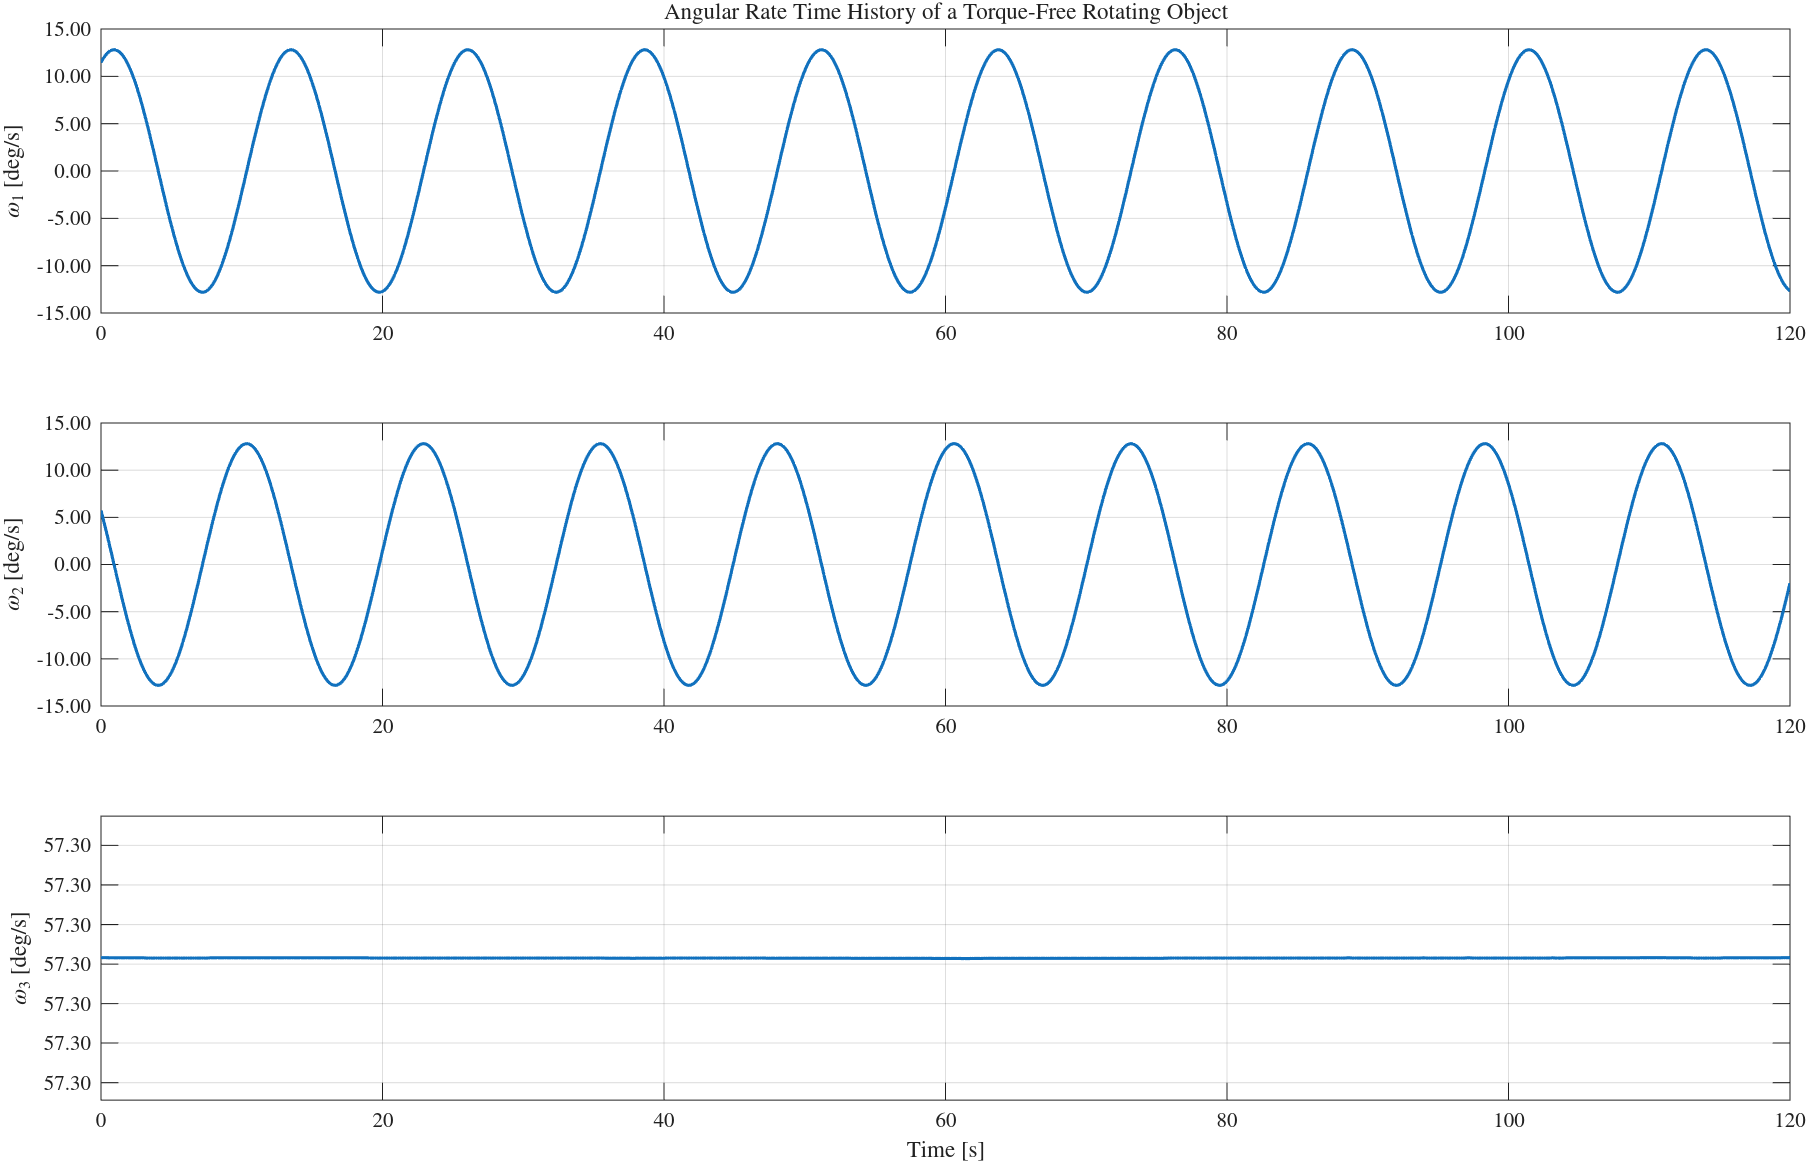
\includegraphics[width=0.85\textwidth]{partf1.png}
		\caption{Time history of the angular rates $\omega_1$, $\omega_2$, and $\omega_3$.}
		\label{fig:f1}
	\end{figure}
	Observe in the plots above that there is an oscillation in the angular rate of the $\hat{\boldsymbol{b}}_1$ and $\hat{\boldsymbol{b}}_2$ directions that appear to act like a $\sin$ or $\cos$ function approximately. Furthermore the $\hat{\boldsymbol{b}}_3$ axis angular rate stays constant to its initial condition. Both of these behaviors are consistent with analytic derivations of $\omega_1(t)$, $\omega_2(t)$, and $\omega_3(t)$ done in part (d).
\end{mdframed}

\subsubsection*{(f.2) Find}
Compute the value of $\boldsymbol{\omega}(t)$ using the analytical solution from part (d.2). Overlay the numerical and analytical solutions. The two should agree closely; discuss any discrepancy observed.\\

\textbf{Analysis/Conclusions:}
To restate, the analytic expressions for $\boldsymbol{\omega}(t)$ stated in (d.2) were:
\begin{equation}
	\begin{split}
		\omega_1(t)&=\omega_{1_0}\cos(K\omega_{3_0}t)+\omega_{2_0}\sin(K\omega_{3_0}t) \\
		\omega_2(t)&=\omega_{2_0}\cos(K\omega_{3_0}t)-\omega_{1_0}\sin(K\omega_{3_0}t) \\
		\omega_3(t)&=\omega_{3_0} \\
		\text{Where: }K&=(I_T-J)/I_T \\
	\end{split}
\end{equation}

Extending the numerical integration code written for (f.2) to also plot the above analytic expressions, the following plots were made:
\begin{mdframed}[linewidth=1pt, innertopmargin=10pt, innerbottommargin=10pt]
	
	\begin{figure}[H]
		\centering
		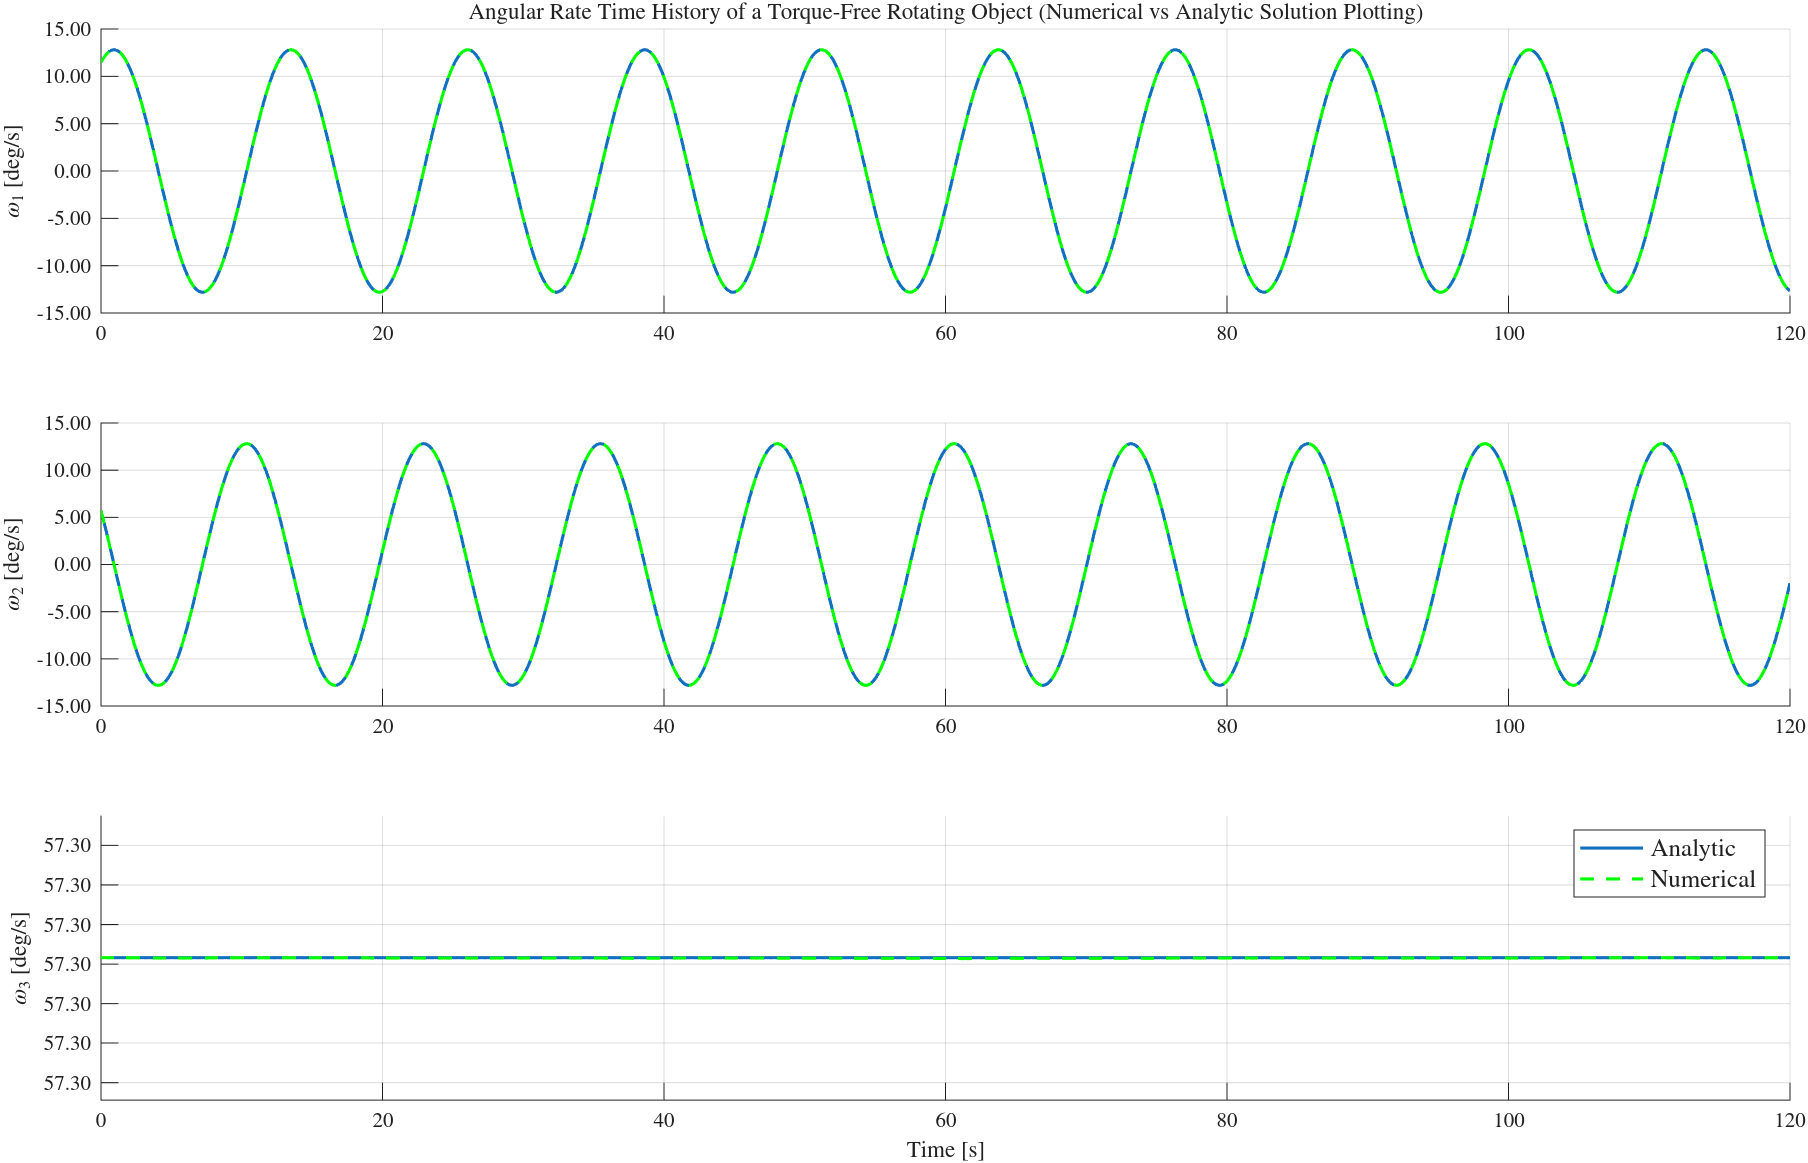
\includegraphics[width=0.85\textwidth]{partf2.png}
		\caption{Time history of the angular rate $\boldsymbol{\omega}$ comparing the analytic solution to a numerical integration of Euler's equations of rotational motion given the same parameters.}
		\label{fig:f2}
	\end{figure}
	It can be seen that the two time histories of $\boldsymbol{\omega}(t)$ from the analytic and numerical approaches follow each other closely. 
	\begin{figure}[H]
		\centering
		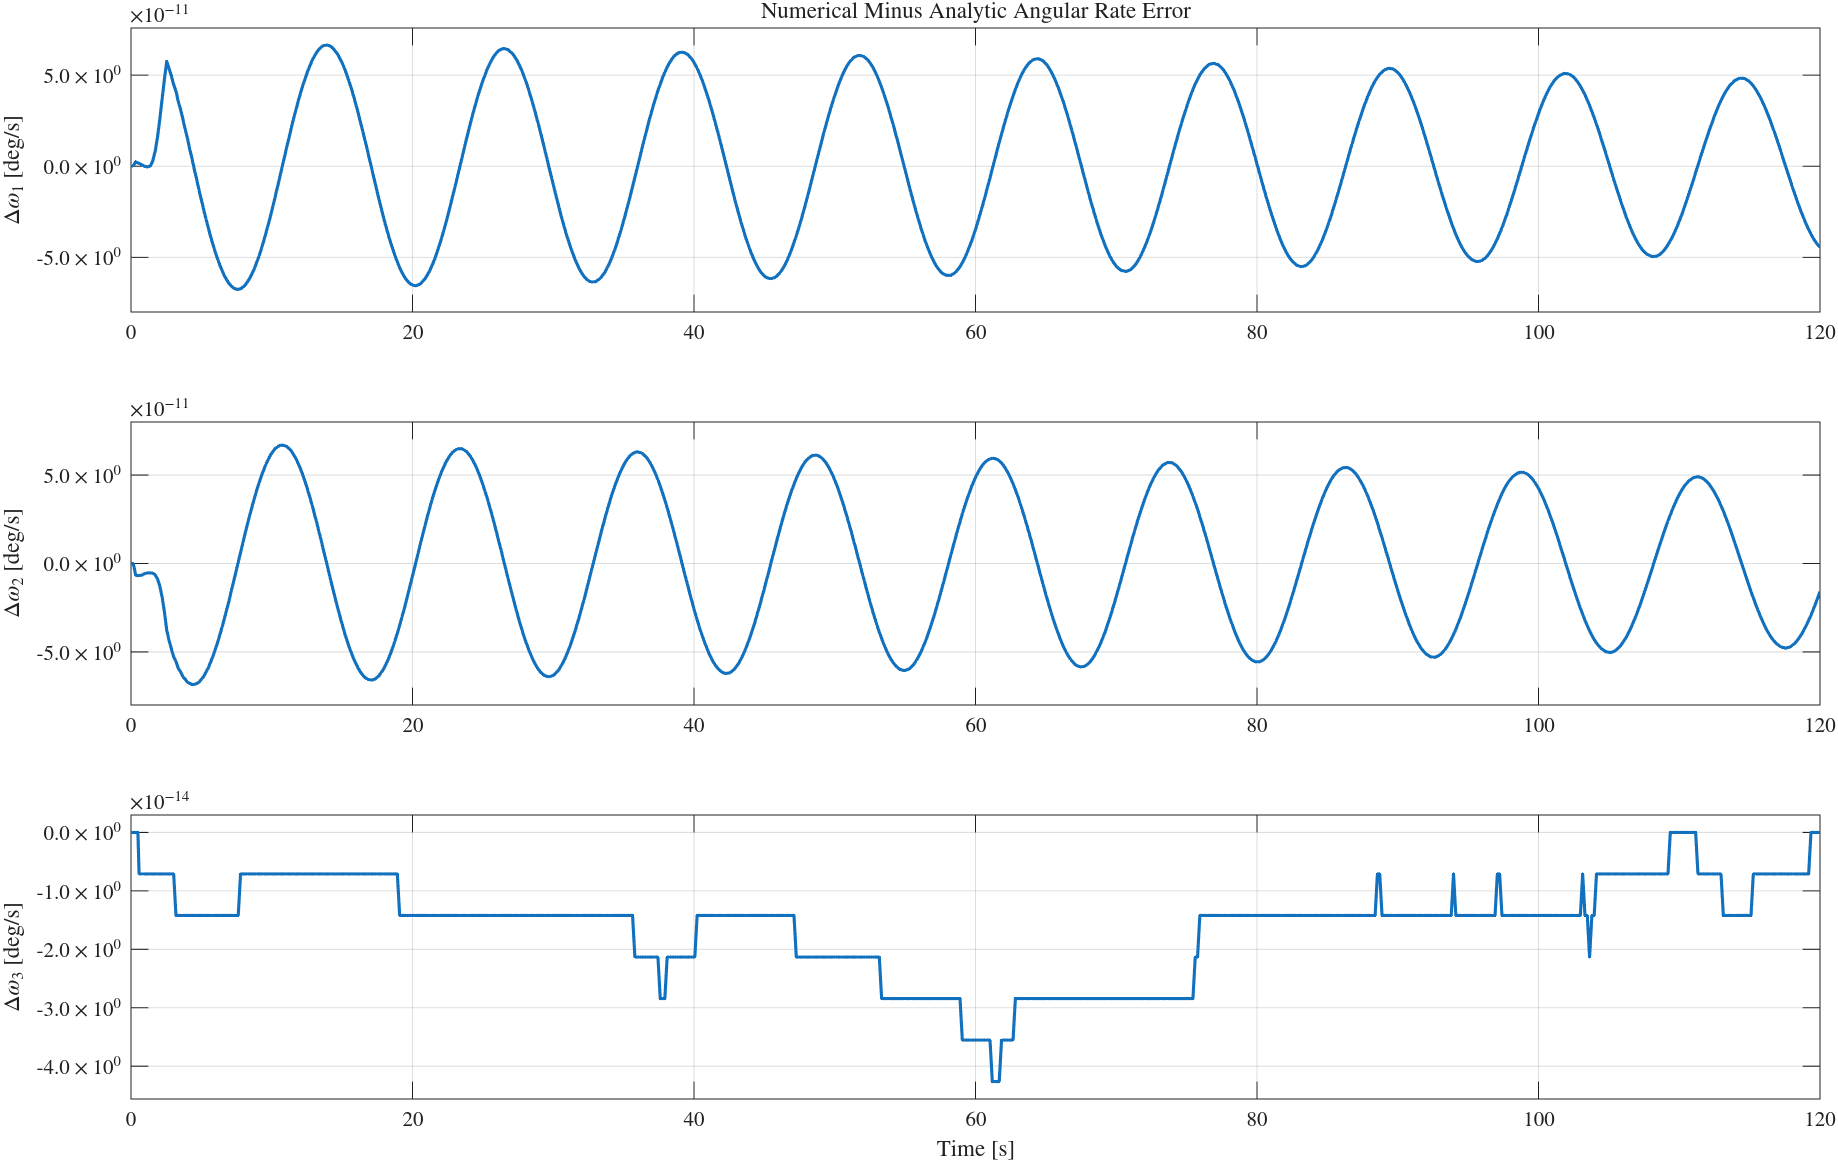
\includegraphics[width=0.85\textwidth]{partf22.png}
		\caption{Plotting difference in $\omega_i(t)$ for all three directions between the analytic and numerical approaches to simulation.}
		\label{fig:f22}
	\end{figure}
	
	When plotting the error of the two methods over time, it can be seen that the difference of $\omega_3$ is exceptionally small with some variance, which is expected because we are effectively comparing the small fluctuations in numerical drift to a true constant. The difference in $\omega_1$ and $\omega_2$ are both three orders of magnitude higher, but still an acceptably low order of magnitude ($10^{-11}$). It is interesting that once the numerical integration gets past the first few oscillations in $\omega_1$ and $\omega_2$, the difference graphs themselves follow a similar oscillation pattern out of phase with the main graphs.
\end{mdframed}

\newpage	
\bibliographystyle{ieeetr}
\bibliography{AAE507HW}
	
\end{document}